\section{Lag Structure and Cross-Correlation Analysis}

\subsection*{Motivation}

The contemporaneous correlation matrix presented in the main report implicitly
assumes that the relationship between CDX IG and its drivers is instantaneous.
In practice, information may propagate with a delay: equity or rates markets may
lead credit by one or more trading days, or credit may adjust sluggishly to
macro shocks. Understanding the lag structure is important both for model
specification (whether lagged regressors would improve fit) and for trading
applications (whether leading indicators exist).

This section examines two complementary diagnostics on daily changes:
\begin{enumerate}
  \item \textbf{Autocorrelation (ACF) and partial autocorrelation (PACF) of
    $\Delta$CDX\,IG} --- to assess persistence or mean-reversion in credit
    spread movements themselves.
  \item \textbf{Cross-correlation functions (CCF)} between each candidate
    driver and $\Delta$CDX\,IG at lags $-20$ to $+20$ days --- to identify
    whether any variable systematically leads or lags CDX IG.
\end{enumerate}

All computations use the \texttt{statsmodels} library. Confidence bands
correspond to the 95\% asymptotic interval $\pm\,1.96 / \sqrt{N}$, where $N$
is the number of observations.

\subsection*{ACF and PACF of CDX IG Daily Changes}

Figure~\ref{fig:acf_pacf} shows the sample autocorrelation and partial
autocorrelation of $\Delta$CDX\,IG up to 20 lags. Shaded bands indicate the
95\% confidence region under the null hypothesis of white noise.

\begin{figure}[H]
  \centering
  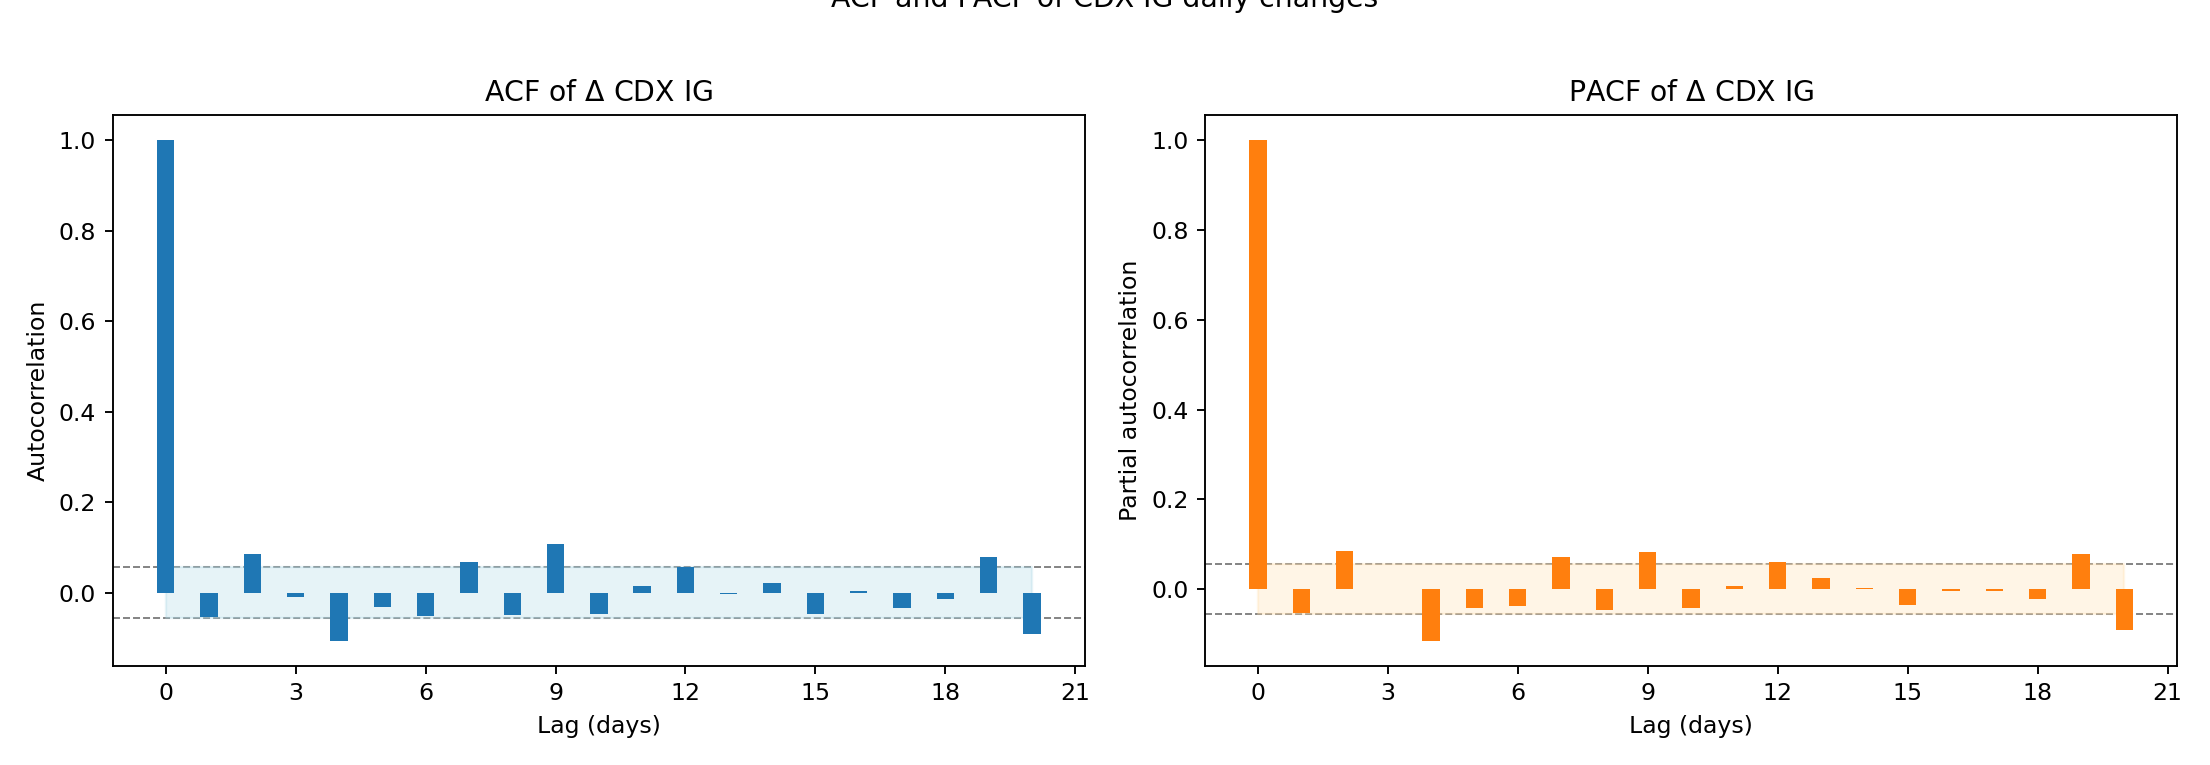
\includegraphics[width=\textwidth]{../../../output/figures/CDX_IG_acf_pacf.png}
  \caption{ACF and PACF of CDX IG daily changes with 95\% confidence bands.}
  \label{fig:acf_pacf}
\end{figure}

A small but statistically significant negative autocorrelation at lag~1 is
consistent with a mild mean-reversion pattern in daily credit spread
changes---i.e.\ a wide day tends to be followed by a slightly narrower day,
and vice versa. Beyond the first few lags the autocorrelation structure is
largely insignificant, suggesting that daily changes are close to white noise
and that an AR(1) or MA(1) component, if included, would capture most of the
serial dependence.

\subsection*{Cross-Correlation with Driver Variables}

Figure~\ref{fig:ccf} presents the cross-correlation function between each
driver and CDX IG daily changes. Positive lags indicate the driver leading CDX
IG; negative lags indicate the driver lagging CDX IG. The dashed lines and
shaded regions mark the 95\% confidence bounds.

\begin{figure}[H]
  \centering
  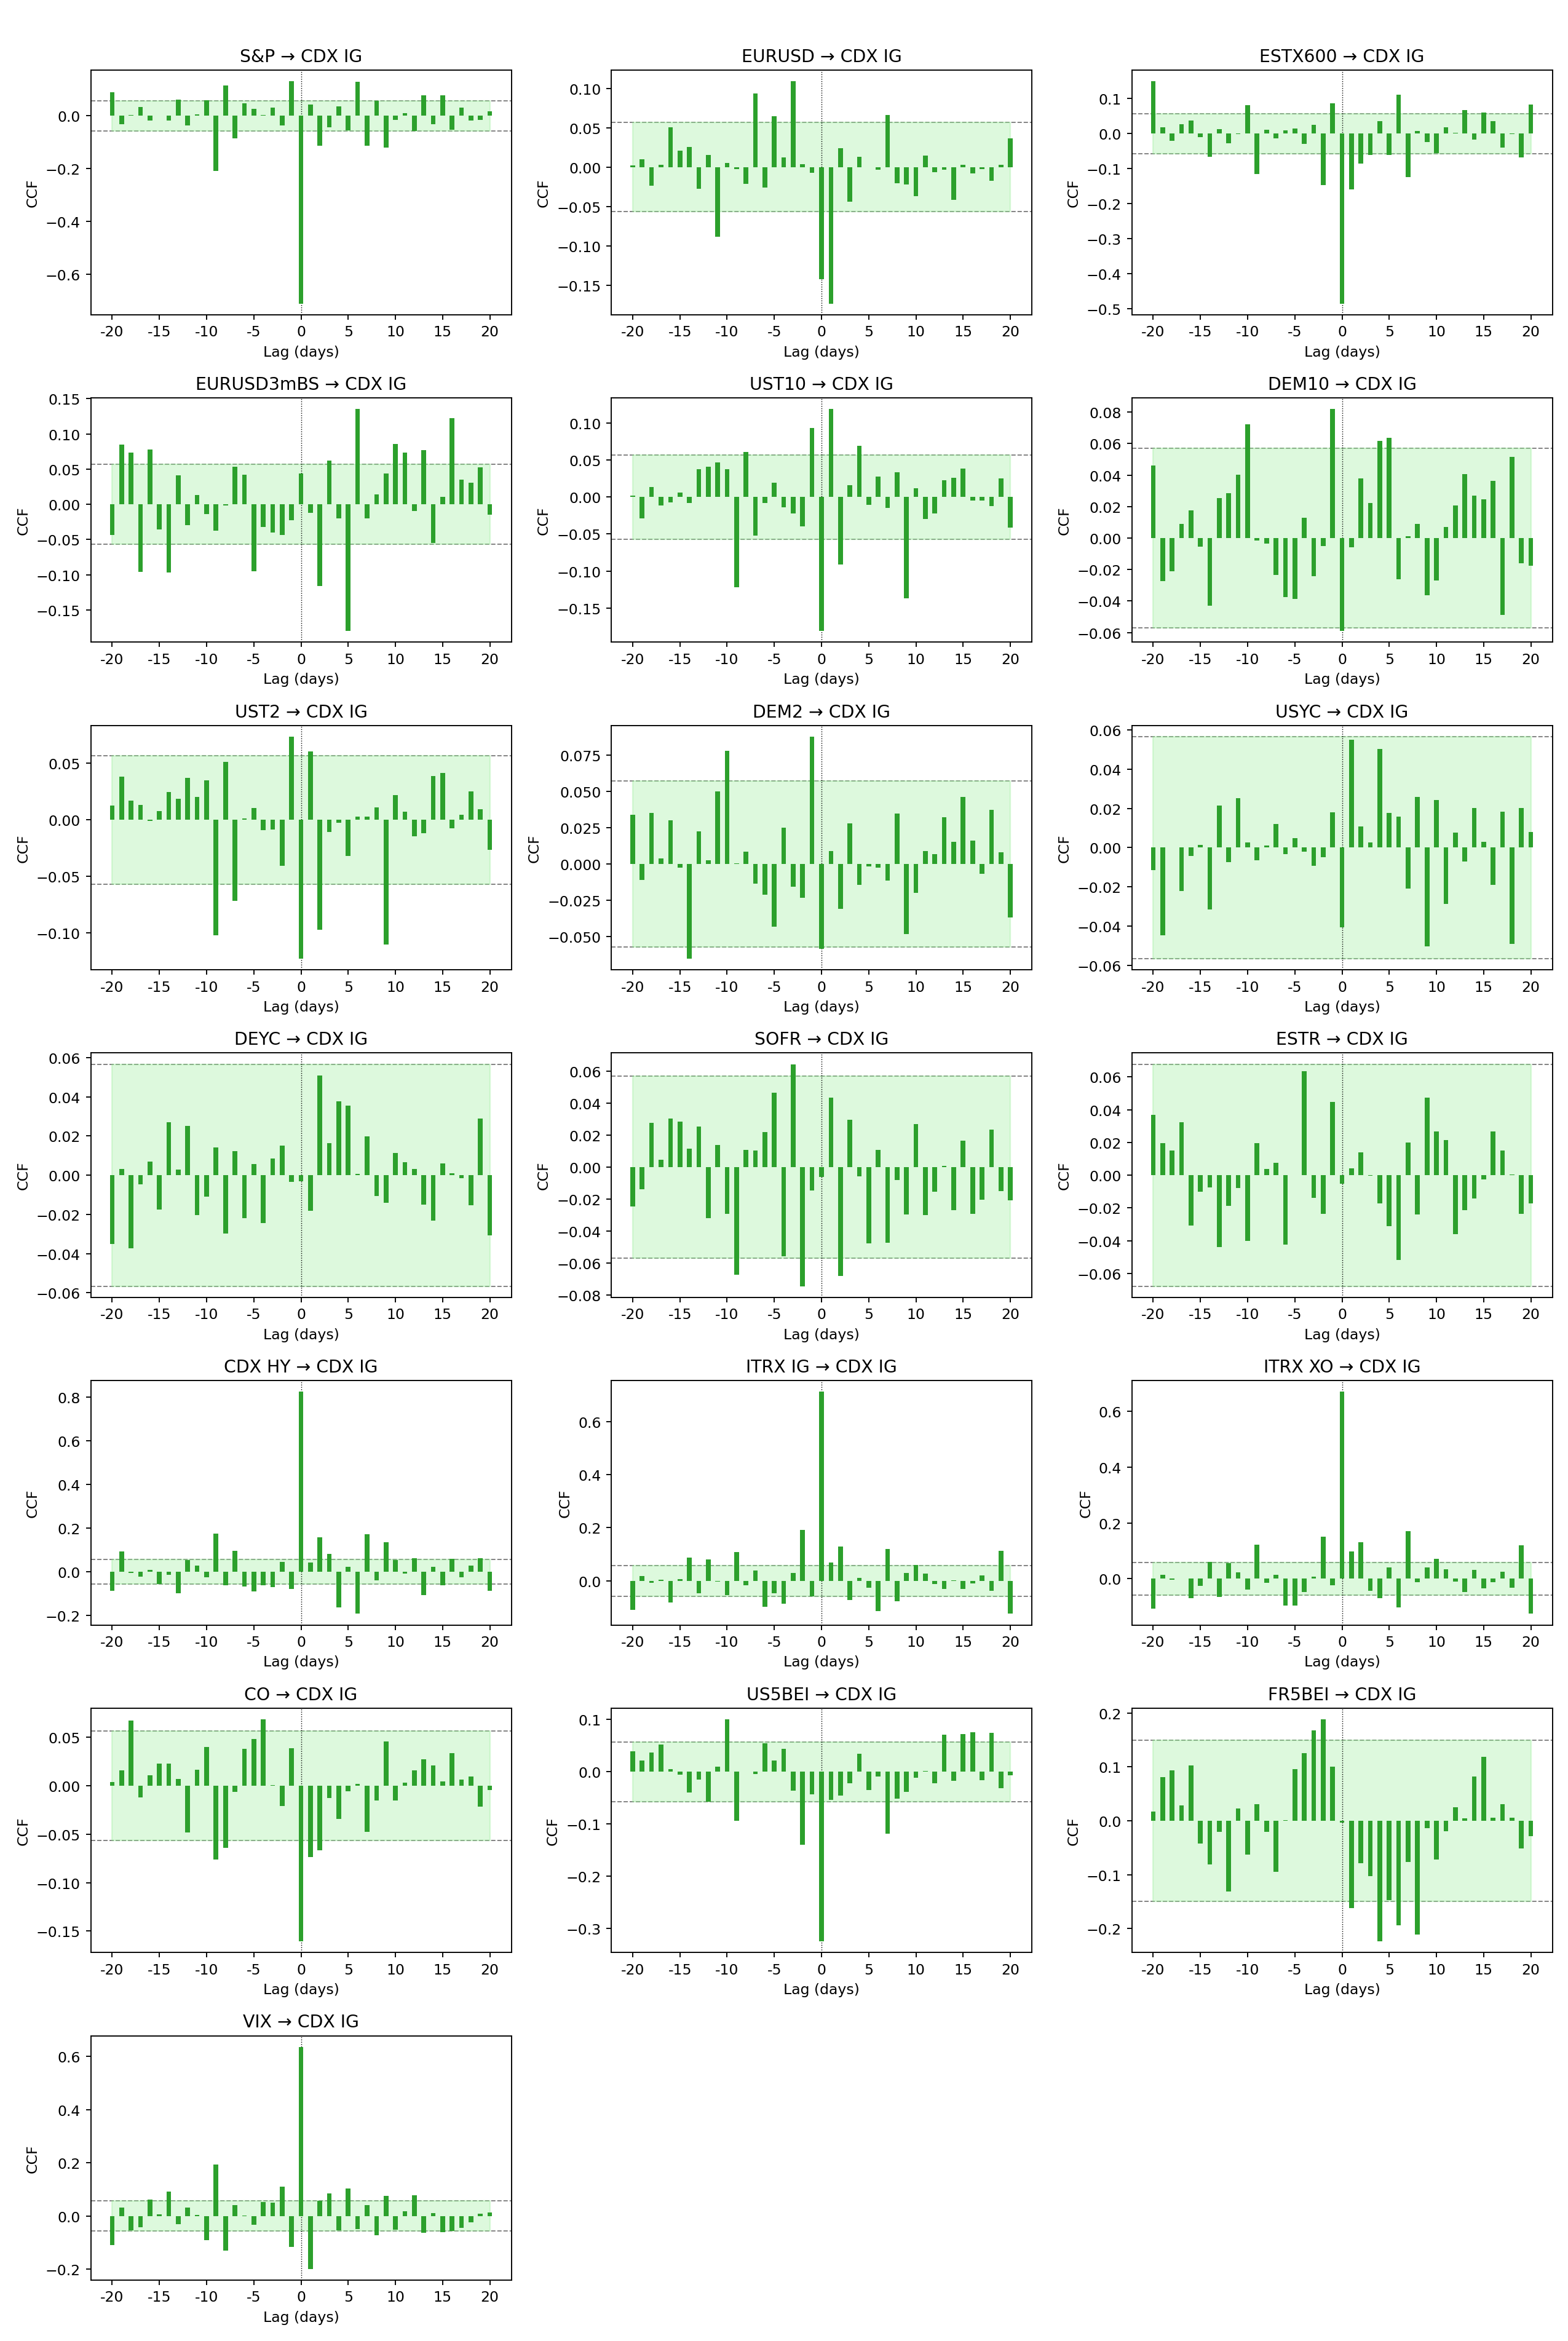
\includegraphics[width=\textwidth]{../../../output/figures/CDX_IG_cross_correlations.png}
  \caption{Cross-correlation functions: driver variables vs CDX IG daily
    changes. Positive lag = driver leads CDX IG.}
  \label{fig:ccf}
\end{figure}

Key observations:

\begin{itemize}
  \item \textbf{Contemporaneous dominance.} For most variables, the strongest
    cross-correlation occurs at lag~0, confirming that the bulk of the
    co-movement is synchronous within the same trading day.

  \item \textbf{VIX and equity indices.} The VIX and S\&P show the highest
    contemporaneous cross-correlations, consistent with the fair-value model
    results in the main report. Any lead--lag structure is small relative to
    the lag-0 signal.

  \item \textbf{European credit indices (ITRX IG, ITRX XO).} These exhibit
    a modest positive cross-correlation at lag~$+1$, reflecting the time-zone
    effect: European markets close before US markets, so European credit
    movements during the same calendar day can appear to ``lead'' CDX IG by
    one observation in end-of-day data.

  \item \textbf{Rates variables (UST10, SOFR, DEM10).} Cross-correlations
    decay rapidly beyond lag~0, indicating no persistent leading or lagging
    relationship with credit spreads at the daily frequency.

  \item \textbf{Crude oil (CO).} The cross-correlation is modest and centred
    at lag~0, with no evidence that oil prices systematically lead credit
    spreads or vice versa over this sample.
\end{itemize}

\subsection*{Implications for Model Specification}

The lag analysis supports the contemporaneous specification adopted in the
main-report fair-value model: the cross-correlations are overwhelmingly
concentrated at lag~0, and including lagged regressors would add model
complexity without material improvement in explanatory power. The mild
lag-1 autocorrelation in CDX IG changes could motivate an AR(1) error
correction term, but its magnitude is small enough that the practical benefit
is limited relative to the added estimation burden.
